\documentclass[11pt,a4paper]{article}

\usepackage[a4paper,margin=1in]{geometry}
\usepackage{amsmath}
\usepackage{amssymb}
\usepackage{booktabs}
\usepackage{array}
\usepackage{longtable}
\usepackage{graphicx}
\usepackage{float}
\usepackage{placeins}
\usepackage{graphicx}
\usepackage{float}
\usepackage{placeins}
\usepackage{hyperref}
\usepackage{enumitem}
\usepackage{hyperref}
\usepackage{enumitem}
\usepackage{titlesec}
\usepackage{listings}
\usepackage{xcolor}

\hypersetup{
colorlinks=true,
linkcolor=blue,
urlcolor=blue
}

\lstset{
language=Python,
basicstyle=\ttfamily\small,
keywordstyle=\color{blue},
commentstyle=\color{green!50!black},
stringstyle=\color{red},
numbers=left,
numberstyle=\tiny,
stepnumber=1,
breaklines=true,
frame=single,
showstringspaces=false
}

\renewcommand{\arraystretch}{1.4}

\begin{document}
\raggedbottom

\setlength{\textfloatsep}{10pt}
\setlength{\floatsep}{8pt}
\setlength{\intextsep}{8pt}

\clubpenalty=10000
\widowpenalty=10000
\displaywidowpenalty=10000

\begin{center}

{\Large \textbf{Shiv Nadar University Chennai}}

\vspace{0.3cm}

\begin{tabular}{|p{4cm}|p{8cm}|p{2cm}|}
\hline
Degree \& Branch &
B.Tech Artificial Intelligence \& Data Science &
Semester V\\
\hline
Subject Code \& Name &
CS3807 -- Deep Learning Laboratory &
AY: 2026--27\\
\hline
\end{tabular}

\vspace{0.7cm}

{\Large \textbf{Experiment 4}}

\vspace{0.2cm}

{\large \textbf{Comparative Study of Deep Convolutional Neural Network Architectures Using Transfer Learning}}

\end{center}

\section*{1. Objective}

The objective of this experiment is to study the evolution of deep convolutional neural network architectures -- LeNet-5, AlexNet, VGG16, GoogleNet and ResNet -- and to understand, in practice, how transfer learning allows a network pretrained on a large dataset such as ImageNet to be repurposed for a new classification task. This is achieved by loading a pretrained ResNet50 backbone, replacing its original classification head with a new one suited to the ten classes of CIFAR-10, training this head while the convolutional base remains frozen, subsequently fine-tuning the last convolutional block of the backbone at a reduced learning rate, and finally evaluating the resulting model using standard classification metrics -- Accuracy, Precision, Recall, F1-score, the Confusion Matrix and the Classification Report -- so that the benefit of fine-tuning over a purely frozen-backbone approach can be measured directly.

\section*{2. Learning Outcomes}

Students will be able to

\begin{enumerate}
\item Explain modern CNN architectures.
\item Differentiate LeNet, AlexNet, VGG16, GoogleNet and ResNet.
\item Implement transfer learning.
\item Fine tune pretrained CNN models.
\item Compare CNN architectures using performance metrics.
\end{enumerate}

\section*{3. Introduction}

Deep Convolutional Neural Networks have become the dominant models for computer vision applications because they automatically learn hierarchical features directly from raw image data, removing the need for handcrafted feature extraction that dominated earlier computer vision pipelines. The evolution of CNN architectures over the past three decades has largely been driven by two competing goals: improving classification accuracy on increasingly difficult benchmarks such as ImageNet, and doing so without a proportional explosion in computational cost or training difficulty. The progression began with LeNet-5, a comparatively shallow network designed for digit recognition, and evolved through AlexNet, VGGNet, GoogleNet and ResNet, each of which introduced a distinct architectural innovation -- ReLU activations and GPU training, uniform small convolution filters, multi-branch inception modules, and residual skip connections respectively -- that addressed a specific limitation of its predecessors and pushed the achievable depth and accuracy of CNNs substantially further.

\section*{4. Background Theory -- Evolution of CNN Architectures}

\subsection*{4.1 LeNet-5}

LeNet-5, proposed by Yann LeCun in 1998, was the first practical convolutional neural network and was designed for handwritten digit recognition. It consists of two convolution layers, two average pooling layers and a small stack of fully connected layers, and it demonstrated for the first time that a network could learn useful image features directly from pixel data rather than relying on manually engineered features. With only around 60 thousand parameters, LeNet-5 trains quickly and remains well suited to constrained tasks such as optical character recognition, though its shallow depth limits how well it generalizes to more complex, natural images such as those in CIFAR-10.

\subsection*{4.2 AlexNet}

AlexNet won the 2012 ImageNet Challenge by a wide margin, reducing the top-5 classification error substantially relative to prior approaches, and is widely credited with reigniting mainstream interest in deep learning. Its major innovations were the use of the ReLU activation function in place of the saturating Sigmoid or Tanh units used previously, Dropout regularization to combat overfitting in its large fully connected layers, and, critically, an implementation split across GPUs that made training a network of roughly 61 million parameters computationally feasible. Data augmentation was also used extensively to artificially expand the effective size of the training set.

\subsection*{4.3 VGG16}

VGG16 demonstrated that stacking many small $3\times3$ convolution filters, rather than using fewer, larger filters as in AlexNet, could outperform larger-filter architectures while increasing overall network depth to 16 weight layers. The uniformity of its $3\times3$ filters throughout the network gives VGG16 a simple, highly regular architecture that is easy to reason about and extend, and its convolutional layers remain a popular choice as a feature extractor for transfer learning, although at 138 million parameters it is considerably more expensive, both in memory and in computation, than the architectures that followed it.

\subsection*{4.4 GoogleNet (Inception Network)}

GoogleNet, proposed by Szegedy \textit{et al.} in 2014, introduced the \textbf{Inception Module}, which performs several convolution operations of different filter sizes in parallel rather than committing to a single kernel size. Specifically, $1\times1$, $3\times3$ and $5\times5$ convolutions and a max pooling branch are applied simultaneously to the same input, and their outputs are concatenated along the channel dimension to yield a multi-scale feature representation at every stage of the network. Crucially, $1\times1$ convolutions are applied before the larger $3\times3$ and $5\times5$ branches purely to reduce the number of input channels first, which sharply reduces both the parameter count and the computational cost of the subsequent larger convolutions. This design allowed GoogleNet to reach a depth of 22 layers while requiring only around 6.8 million parameters, substantially fewer than either AlexNet or VGG16, while achieving better classification performance than both.

\subsection*{4.5 ResNet}

Increasing the depth of a CNN indiscriminately tends to cause the \textbf{vanishing gradient problem}, in which gradients computed during backpropagation shrink as they are propagated back through many layers, making the earliest layers of a very deep network difficult or impossible to train effectively. ResNet, proposed by He \textit{et al.} in 2015, solves this issue using \textbf{skip (residual) connections}, which allow the input to a block of layers to be added directly to that block's output, giving gradients an unimpeded path to flow backward through the network regardless of its depth. Rather than requiring a stack of layers to learn the full underlying mapping $H(x)$ directly, ResNet reformulates the problem so that the stack instead learns the residual

\[
F(x) = H(x) - x
\]

so that the block's actual output is recovered as

\[
Output = F(x) + x
\]

where $F(x)$ is the residual mapping learned by the convolutional layers within the block and $x$ is the identity mapping carried forward by the skip connection. This reformulation makes it considerably easier for a block to learn an identity mapping when that is the optimal behaviour, since the residual branch need only learn to output zero, rather than having to learn the identity function exactly through a stack of nonlinear layers.

\begin{center}
Input $\rightarrow$ Conv $\rightarrow$ Conv $\rightarrow (+) \rightarrow$ Output
\end{center}
\begin{center}
\textit{(Residual Block: the skip connection carries the Input directly to the addition node)}
\end{center}

\vspace{0.15cm}

The advantages of this design are that it eliminates vanishing gradients even in very deep networks, enables architectures of 50, 101 or more layers to be trained successfully, leads to faster convergence during training, and achieves higher ImageNet accuracy than any of the architectures preceding it. ResNet50, the 50-layer variant used later in this experiment, uses roughly 25.6 million parameters -- fewer than either AlexNet or VGG16 despite being substantially deeper, which is a direct consequence of its efficient bottleneck block design.

\subsection*{4.6 Dilated Convolution}

Dilated convolution, also called atrous convolution, increases the effective receptive field of a convolution kernel without increasing the number of trainable parameters, by inserting gaps between the kernel's individual weights. The spacing between kernel elements is controlled by the dilation rate $D$: for a standard convolution $D=1$, so the kernel weights are contiguous, whereas for a dilated convolution $D>1$ and zeros are effectively inserted between weights, for example transforming a compact $3\times3$ kernel such as

\[
\begin{bmatrix}
1 & 2 & 3\\
4 & 5 & 6\\
7 & 8 & 9
\end{bmatrix}
\rightarrow
\begin{bmatrix}
1 & 0 & 2\\
0 & 3 & 0\\
4 & 0 & 5
\end{bmatrix}
\]

so that the kernel now spans a larger region of the input while still applying the same number of multiplications. This is particularly useful in tasks such as semantic segmentation, medical image analysis, satellite imagery interpretation and object localization, where a large receptive field is needed to capture context without discarding spatial resolution through pooling.

\subsection*{4.7 Transpose Convolution}

Transpose convolution increases the spatial dimensions of a feature map rather than reducing them. Whereas ordinary pooling operations discard spatial information to shrink a feature map, transpose convolution performs a learnable form of upsampling, in which the network itself learns how to expand a low-resolution feature map back to a higher resolution. This operation underlies applications such as image super-resolution, autoencoder decoders, Generative Adversarial Networks, general image generation and the decoder pathway of semantic segmentation networks, all of which require projecting a compressed representation back into a full-resolution image or feature map.

\section*{5. Comparison of Architectures}

\begin{center}
\begin{tabular}{|p{3cm}|c|c|p{5cm}|}
\hline
\textbf{Architecture} & \textbf{Depth} & \textbf{Parameters} & \textbf{Main Contribution}\\
\hline
LeNet-5 & 7 & 60K & First CNN\\
\hline
AlexNet & 8 & 61M & ReLU + Dropout\\
\hline
VGG16 & 16 & 138M & Deep $3\times3$ filters\\
\hline
GoogleNet & 22 & 6.8M & Inception Modules\\
\hline
ResNet50 & 50 & 25.6M & Residual Learning\\
\hline
\end{tabular}
\end{center}

\vspace{0.15cm}

This table makes clear that depth alone is not what determines a network's parameter count: GoogleNet, despite being the second-deepest network in the table at 22 layers, has by far the fewest parameters of the group, a direct consequence of its Inception module's use of $1\times1$ convolutions to reduce channel counts before more expensive operations. ResNet50, although the deepest architecture listed at 50 layers, requires fewer parameters than both AlexNet and VGG16, illustrating that the residual bottleneck design used throughout ResNet is considerably more parameter-efficient per layer than either AlexNet's large fully connected layers or VGG16's uniform stack of full-width $3\times3$ convolutions.

\section*{6. Transfer Learning Explanation}

Transfer learning utilizes a CNN that has already been pretrained on a large dataset such as ImageNet, which contains over a million labelled images across a thousand categories, so that the general-purpose visual features -- edges, textures, shapes and object parts -- it has already learned can be reused on a new, smaller dataset rather than being learned again from scratch. Instead of training an entire network from randomly initialized weights, the standard transfer learning workflow proceeds as follows: first, a pretrained model is loaded together with its ImageNet weights; its original classification layer, which was designed for 1,000 ImageNet categories, is then removed; the remaining convolutional base is frozen so that its pretrained weights are not disturbed during the earliest phase of training; new Dense layers suited to the target task are added on top of the frozen base; this new classification head is trained while the base remains frozen; and finally, selected convolutional layers -- typically the last block, which encodes the most task-specific features -- are unfrozen and fine-tuned at a reduced learning rate to adapt the pretrained features more closely to the new dataset. This workflow is illustrated conceptually as

\begin{center}
ImageNet Pretrained Model $\rightarrow$ Remove Classifier $\rightarrow$ Freeze Layers $\rightarrow$ Add Dense Layers $\rightarrow$ Fine Tune $\rightarrow$ Prediction
\end{center}

The advantages of this approach are faster convergence, since the network does not need to relearn low-level features from scratch; higher accuracy on small datasets, since the pretrained weights already encode a rich, general-purpose visual representation; reduced training time overall; and lower computational cost compared with training a comparably deep network entirely from random initialization.

\section*{7. Dataset Description}

The experiment uses the \textbf{CIFAR-10 Dataset}, loaded from the Hugging Face Hub via the \texttt{datasets} library rather than \texttt{torchvision.datasets.CIFAR10}, so that each example is exposed as a dictionary containing a PIL image under the \texttt{img} key and an integer label under the \texttt{label} key.

\vspace{0.3cm}

\begin{center}
\begin{tabular}{|p{5cm}|p{7cm}|}
\hline
\textbf{Property} & \textbf{Value}\\
\hline
Dataset Name & CIFAR-10\\
\hline
Source & Hugging Face Hub, \texttt{uoft-cs/cifar10}\\
\hline
Training Images & 50{,}000\\
\hline
Testing Images & 10{,}000\\
\hline
Original Image Size & $32 \times 32 \times 3$ (RGB)\\
\hline
Resized Image Size & $224 \times 224 \times 3$ (RGB)\\
\hline
Target Classes & 10\\
\hline
Learning Type & Supervised Learning\\
\hline
Problem Type & Multi-class Image Classification\\
\hline
\end{tabular}
\end{center}

\vspace{0.15cm}
\textbf{Target Classes}

\begin{center}
\begin{tabular}{|c|p{9cm}|}
\hline
\textbf{Class Label} & \textbf{Description}\\
\hline
0 & airplane\\
\hline
1 & automobile\\
\hline
2 & bird\\
\hline
3 & cat\\
\hline
4 & deer\\
\hline
5 & dog\\
\hline
6 & frog\\
\hline
7 & horse\\
\hline
8 & ship\\
\hline
9 & truck\\
\hline
\end{tabular}
\end{center}

\vspace{0.3cm}

Since the ResNet50 backbone used in this experiment expects the $224\times224$ input resolution that ImageNet models were originally trained on, every $32\times32$ CIFAR-10 image was resized to $224\times224$ as part of the transform pipeline, in addition to being normalized using the standard ImageNet channel-wise mean and standard deviation. This upsampling is a deliberate and necessary deviation from the raw CIFAR-10 format: without it, the pretrained convolutional filters -- tuned to the spatial scale of ImageNet images -- would not be applicable to the much smaller native CIFAR-10 resolution, and the benefit of transfer learning would be lost.

\section*{8. Experimental Procedure}

The experiment was carried out using Python and PyTorch in Google Colab, with automatic detection of the available compute device (CUDA GPU or CPU) and a fixed random seed for reproducibility.

\begin{center}
\begin{tabular}{|p{5cm}|p{7cm}|}
\hline
\textbf{Property} & \textbf{Value}\\
\hline
Device Used & CUDA GPU\\
\hline
Random Seed & 42\\
\hline
Framework & PyTorch\\
\hline
Backbone & ResNet50 (\texttt{torchvision.models.resnet50}), ImageNet pretrained\\
\hline
\end{tabular}
\end{center}

\vspace{0.3cm}

\subsection*{Task 1: Dataset Preparation}

CIFAR-10 was loaded from the Hugging Face Hub and wrapped in a custom PyTorch \texttt{Dataset} class that applies the resize-to-$224\times224$, tensor-conversion and ImageNet-normalization transform pipeline to every image. Ten representative sample images were displayed with their true class names, and the training and testing dataset dimensions were printed.

\subsection*{Task 2: Transfer Learning Setup}

A ResNet50 model was loaded with pretrained ImageNet weights, its convolutional base was frozen, and its original 1000-class classification layer was replaced with a new head consisting of the existing Global Average Pooling layer followed by a Dense (Linear) layer with ReLU activation and a final 10-unit output layer, with Softmax realized implicitly via the Cross-Entropy loss.

\subsection*{Task 3: Model Training (Frozen Backbone)}

The new classification head was trained for 10 epochs using the Adam optimizer with a learning rate of 0.001, a batch size of 32 and the Cross-Entropy loss function, while every convolutional layer of the ResNet50 backbone remained frozen.

\subsection*{Task 4: Fine-Tuning}

The last convolutional block of ResNet50 (\texttt{layer4}) was unfrozen, and the model was trained for a further 5 epochs at a reduced learning rate of 0.0001, so that the pretrained backbone weights could adapt to CIFAR-10 without being disrupted too aggressively. The classification accuracy before and after fine-tuning was then compared directly.

\subsection*{Task 5: Model Evaluation}

The fine-tuned model was evaluated on the untouched testing set of 10,000 images. Accuracy, macro-averaged Precision, Recall and F1-score, the per-class Classification Report and the Confusion Matrix were computed, and a sample of misclassified test images was inspected directly.

\section*{9. Model Architecture (ResNet50 Transfer-Learning Head)}

The transfer-learning model implemented for this experiment consists of the full ResNet50 convolutional backbone, pretrained on ImageNet, followed by a new classification head, as summarized below.

\begin{center}
\begin{tabular}{|p{5.5cm}|p{9.5cm}|}
\hline
\textbf{Layer} & \textbf{Configuration}\\
\hline
Backbone & ResNet50 convolutional base (ImageNet pretrained, frozen during Task 3)\\
\hline
Global Average Pooling & ResNet50's existing adaptive average pooling layer\\
\hline
FC1 & Linear($2{,}048 \rightarrow 256$), ReLU\\
\hline
Dropout & Dropout($p=0.3$)\\
\hline
FC2 (Output) & Linear($256 \rightarrow 10$), Softmax (via Cross-Entropy loss)\\
\hline
\end{tabular}
\end{center}

\vspace{0.15cm}

The network was compiled with the Cross-Entropy loss function. During Task 3, only the parameters of the new classification head (FC1 and FC2) were trainable, while during Task 4 the parameters of \texttt{layer4}, the final residual block of the ResNet50 backbone, were additionally unfrozen and trained alongside the head, allowing the deepest, most task-specific convolutional filters to adapt to the visual characteristics of CIFAR-10.

\section*{10. Hyperparameter Study}

\begin{center}
\begin{tabular}{|c|c|}
\hline
\textbf{Hyperparameter} & \textbf{Values}\\
\hline
Learning Rate & 0.001, 0.0001\\
\hline
Batch Size & 16, 32, 64\\
\hline
Epochs & 10, 20\\
\hline
Optimizer & Adam, SGD\\
\hline
Dense Units & 128, 256\\
\hline
Frozen Layers & All, Partial\\
\hline
\end{tabular}
\end{center}

\vspace{0.15cm}

Of this grid, only a single configuration was actually trained in this experiment -- a learning rate of 0.001 with 10 frozen-backbone epochs followed by a learning rate of 0.0001 for 5 fine-tuning epochs, a batch size of 32, the Adam optimizer, 256 dense units, and partially frozen layers (\texttt{layer4} unfrozen during fine-tuning) -- and it is marked below as the reference row against which the remaining, unrun configurations are listed for completeness.

\begin{center}
\begin{tabular}{|p{3.8cm}|c|c|c|c|c|p{2.2cm}|c|}
\hline
\textbf{Configuration} & \textbf{LR} & \textbf{Batch} & \textbf{Epochs} & \textbf{Optim.} & \textbf{Dense} & \textbf{Frozen Layers} & \textbf{Test Acc.}\\
\hline
Actually Trained (this run) & 0.001 & 32 & 10 & Adam & 256 & Partial (layer4) & 90.08\%\\
\hline
LR = 0.0001, Batch = 32 & 0.0001 & 32 & 10 & Adam & 256 & Not run & --\\
\hline
Batch = 16 & 0.001 & 16 & 10 & Adam & 256 & Not run & --\\
\hline
Batch = 64 & 0.001 & 64 & 10 & Adam & 256 & Not run & --\\
\hline
Epochs = 20 & 0.001 & 32 & 20 & Adam & 256 & Not run & --\\
\hline
Optimizer = SGD & 0.001 & 32 & 10 & SGD & 256 & Not run & --\\
\hline
Dense Units = 128 & 0.001 & 32 & 10 & Adam & 128 & Not run & --\\
\hline
Frozen Layers = All & 0.001 & 32 & 10 & Adam & 256 & Not run & --\\
\hline
\end{tabular}
\end{center}

\section*{11. Parameter Calculation / Parameter Counts}

The total and trainable parameter counts of the transfer-learning model were printed directly by PyTorch at each stage of the experiment.

\begin{center}
\begin{tabular}{|p{7cm}|p{5cm}|}
\hline
\textbf{Stage} & \textbf{Trainable Parameters}\\
\hline
Total Parameters (entire model) & 24{,}035{,}146\\
\hline
Trainable Parameters (Task 3, frozen backbone) & 527{,}114\\
\hline
Frozen Parameters (Task 3, frozen backbone) & 23{,}508{,}032\\
\hline
Trainable Parameters (Task 4, after unfreezing layer4) & 15{,}491{,}850\\
\hline
\end{tabular}
\end{center}

\vspace{0.15cm}

During the frozen-backbone phase, only 527{,}114 of the model's 24{,}035{,}146 total parameters -- roughly 2.2\% -- were trainable, confirming that almost the entire ResNet50 convolutional base was successfully held fixed at its pretrained ImageNet weights while only the new classification head was updated. Once \texttt{layer4} was unfrozen for fine-tuning, the trainable parameter count rose sharply to 15{,}491{,}850, close to two-thirds of the total model, reflecting the fact that ResNet50's final residual block, which contains its widest and most numerous filters, accounts for the large majority of the backbone's own parameter budget.

\section*{12. Experimental Results}

\subsection*{12.1 Before vs After Fine-Tuning}

\begin{center}
\begin{tabular}{|p{6cm}|c|c|c|c|}
\hline
\textbf{Stage} & \textbf{Train Acc.} & \textbf{Val Acc.} & \textbf{Train Loss} & \textbf{Val Loss}\\
\hline
Frozen Backbone (Final Epoch, 10) & 84.59\% & 82.89\% & 0.4388 & 0.4952\\
\hline
Fine-Tuned (Final Epoch, 5) & 98.68\% & 90.08\% & 0.0402 & 0.3536\\
\hline
\end{tabular}
\end{center}

\vspace{0.15cm}

Fine-tuning the last convolutional block produced a substantial improvement over the frozen-backbone baseline: validation accuracy rose from 82.89\% to 90.08\%, a gain of over 7 percentage points, in only 5 additional epochs, while validation loss fell from 0.4952 to 0.3536. Training accuracy also rose sharply, from 84.59\% to 98.68\%, and training loss fell from 0.4388 to a very low 0.0402, indicating that once \texttt{layer4} was unfrozen the model was able to fit the training data almost perfectly. The frozen-backbone phase took 2{,}265.73 seconds to complete 10 epochs, while fine-tuning took a further 1{,}449.56 seconds for 5 epochs, giving a combined total training time of 3{,}715.28 seconds.

\subsection*{12.2 Test Set Evaluation}

\begin{center}
\begin{tabular}{|p{6cm}|c|}
\hline
\textbf{Metric} & \textbf{Value}\\
\hline
Test Accuracy & 90.08\%\\
\hline
Precision (macro) & 90.18\%\\
\hline
Recall (macro) & 90.08\%\\
\hline
F1-Score (macro) & 90.07\%\\
\hline
\end{tabular}
\end{center}

\vspace{0.15cm}

\begin{center}
\begin{tabular}{|p{3cm}|c|c|c|c|}
\hline
\textbf{Class} & \textbf{Precision} & \textbf{Recall} & \textbf{F1-Score} & \textbf{Support}\\
\hline
airplane & 0.92 & 0.89 & 0.90 & 1{,}000\\
\hline
automobile & 0.96 & 0.93 & 0.94 & 1{,}000\\
\hline
bird & 0.92 & 0.86 & 0.89 & 1{,}000\\
\hline
cat & 0.82 & 0.82 & 0.82 & 1{,}000\\
\hline
deer & 0.89 & 0.89 & 0.89 & 1{,}000\\
\hline
dog & 0.85 & 0.88 & 0.86 & 1{,}000\\
\hline
frog & 0.89 & 0.95 & 0.92 & 1{,}000\\
\hline
horse & 0.95 & 0.89 & 0.92 & 1{,}000\\
\hline
ship & 0.89 & 0.97 & 0.93 & 1{,}000\\
\hline
truck & 0.93 & 0.94 & 0.93 & 1{,}000\\
\hline
\textbf{Macro/Weighted Avg} & \textbf{0.90} & \textbf{0.90} & \textbf{0.90} & \textbf{10{,}000}\\
\hline
\end{tabular}
\end{center}

\vspace{0.15cm}

The per-class results show automobile (96\% precision, 93\% recall) and ship (89\% precision, 97\% recall) as the most reliably classified categories, alongside strong performance on truck and horse. The weakest class by a clear margin is cat, at only 82\% precision and 82\% recall, with dog also comparatively weak at 85\% precision and 88\% recall -- the same cat/dog confusion pattern that is a well-known difficulty in CIFAR-10 classification, since the two classes share broadly similar body shapes, fur textures and typical backgrounds.

\subsection*{12.3 Comparison of CNN Architectures}

\begin{center}
\begin{tabular}{|p{2.8cm}|c|c|p{2.8cm}|p{3cm}|}
\hline
\textbf{Model} & \textbf{Parameters} & \textbf{Accuracy (\%)} & \textbf{Training Time} & \textbf{Source}\\
\hline
LeNet-5 & 60K & -- & -- & Literature\\
\hline
AlexNet & 61M & -- & -- & Literature\\
\hline
VGG16 & 138M & -- & -- & Literature\\
\hline
GoogleNet & 6.8M & -- & -- & Literature\\
\hline
ResNet50 & 24{,}035{,}146 & 90.08 & 3{,}715.28 s & Measured (this run)\\
\hline
\end{tabular}
\end{center}

\vspace{0.15cm}

Since only ResNet50 was actually trained in this experiment, it is the only row in this table with measured accuracy and training-time figures; the remaining rows reproduce the literature parameter counts from Section 5 for reference and are not directly comparable in accuracy or training time, since LeNet-5, AlexNet, VGG16 and GoogleNet were not trained on CIFAR-10 in this experiment. Notably, the transfer-learning ResNet50 model's total parameter count of 24,035,146 is close to, but slightly lower than, the 25.6M figure typically quoted for the base ResNet50 architecture, since the original 1000-class ImageNet classification layer (which contributes just over 2 million parameters) was removed and replaced with the smaller 256-unit head used in this experiment.

\section*{13. Plots and Interpretation}

\subsection*{13.1 Sample Images}

\begin{figure}[H]
\centering
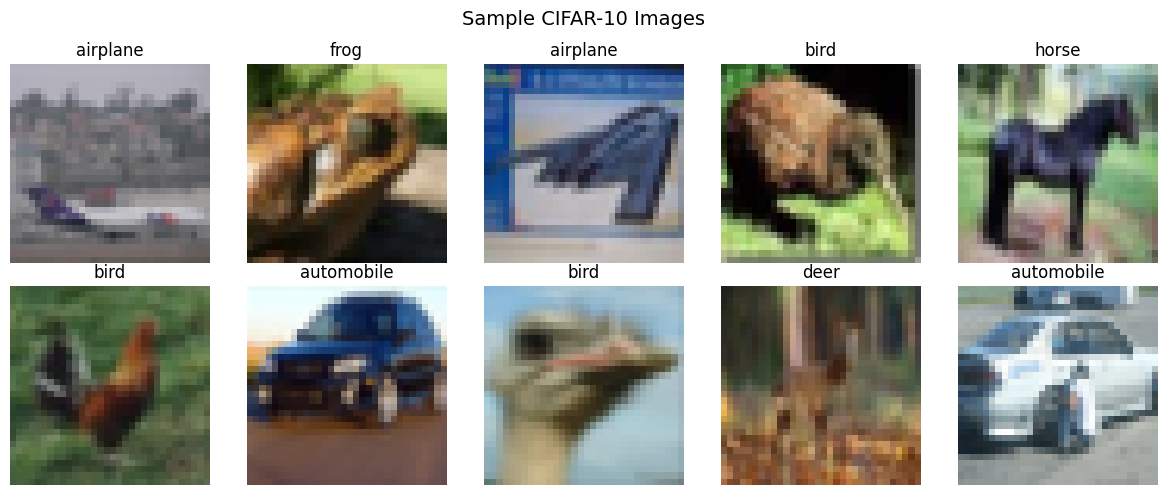
\includegraphics[width=0.95\textwidth]{plot1.png}
\caption{Ten Sample Images from the CIFAR-10 Dataset with True Class Labels}
\end{figure}

The sample images span both vehicles (airplane, automobile) and animals (frog, bird, horse, deer), each shown at low native resolution against a variety of natural backgrounds. Several images, such as the frog and the ostrich labelled ``bird'', show that even at $32\times32$ resolution, distinguishing certain animal classes visually is genuinely difficult, foreshadowing some of the confusion later observed between visually related animal categories in the confusion matrix.

\vspace{0.15cm}

\subsection*{13.2 Training Accuracy (Frozen Backbone)}

\begin{figure}[H]
\centering
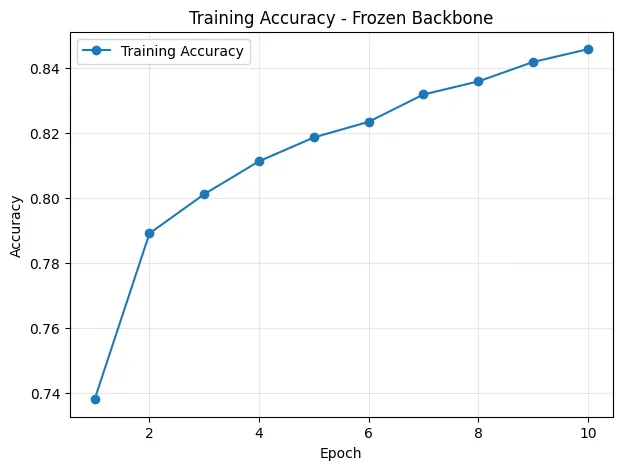
\includegraphics[width=0.75\textwidth]{plot2.png}
\caption{Training Accuracy vs Epoch, Frozen Backbone}
\end{figure}

Training accuracy rises steadily and smoothly across all 10 frozen-backbone epochs, from 73.80\% in the first epoch to 84.59\% by the tenth, with the steepest gains occurring in the first two epochs before the curve begins to flatten. This smooth, well-behaved rise, without the erratic jumps sometimes seen when training an entire network from scratch, reflects the fact that only the small classification head is being optimized here, on top of already-powerful pretrained features.

\vspace{0.15cm}

\subsection*{13.3 Validation Accuracy (Frozen Backbone)}

\begin{figure}[H]
\centering
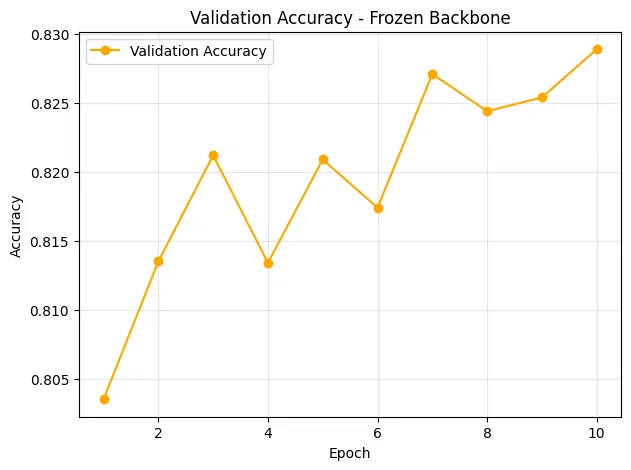
\includegraphics[width=0.75\textwidth]{plot3.png}
\caption{Validation Accuracy vs Epoch, Frozen Backbone}
\end{figure}

Validation accuracy climbs from 80.35\% to 82.89\% over the 10 frozen-backbone epochs, with some mild non-monotonic fluctuation around epochs 4 and 6 rather than a perfectly smooth increase. Unlike the overfitting pattern observed in Experiment 3, validation accuracy here tracks training accuracy fairly closely throughout, and does not decline in later epochs, indicating that the frozen ResNet50 backbone provides features general enough that the small trainable head does not overfit within this training budget.

\vspace{0.15cm}

\subsection*{13.4 Training Loss (Frozen Backbone)}

\begin{figure}[H]
\centering
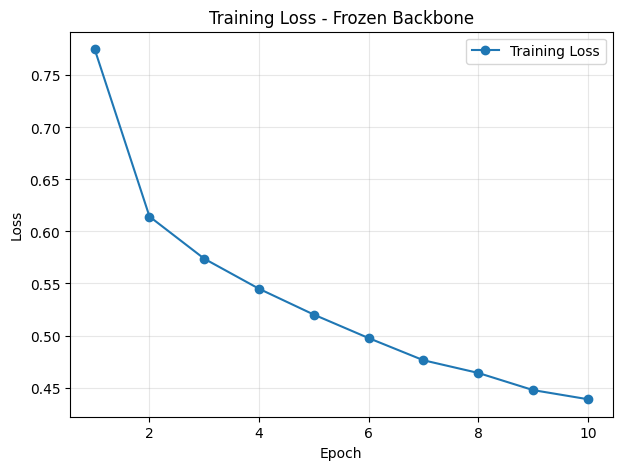
\includegraphics[width=0.75\textwidth]{plot4.png}
\caption{Training Loss vs Epoch, Frozen Backbone}
\end{figure}

Training loss falls sharply from 0.7751 in the first epoch to 0.6143 in the second, before continuing to decrease more gradually to 0.4388 by the tenth epoch. The steep initial drop is typical of transfer learning, since the randomly initialized classification head starts far from a good solution while the frozen backbone already supplies strong, discriminative features, so the head converges quickly once training begins.

\vspace{0.15cm}

\subsection*{13.5 Validation Loss (Frozen Backbone)}

\begin{figure}[H]
\centering
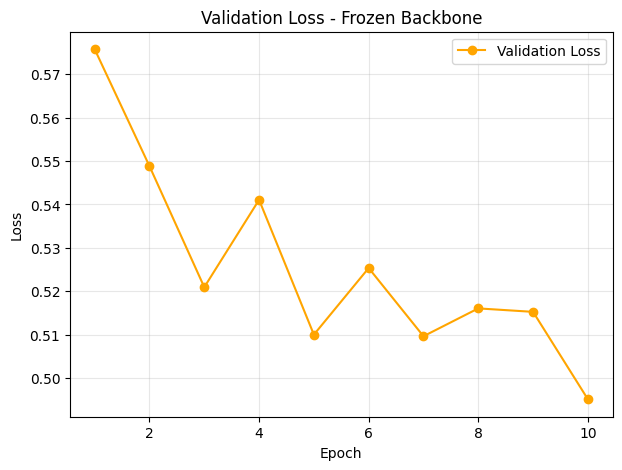
\includegraphics[width=0.75\textwidth]{plot5.png}
\caption{Validation Loss vs Epoch, Frozen Backbone}
\end{figure}

Validation loss falls from 0.5757 to a low of 0.4952 by the tenth epoch, but the curve is visibly noisier than the training loss curve, rising briefly around epochs 4 and 6 before falling again. This mild fluctuation, without any sustained upward trend, is consistent with the validation accuracy behaviour in Section 13.3 and further supports the conclusion that the frozen-backbone model is not yet overfitting within these 10 epochs.

\vspace{0.15cm}

\subsection*{13.6 Confusion Matrix}

\begin{figure}[H]
\centering
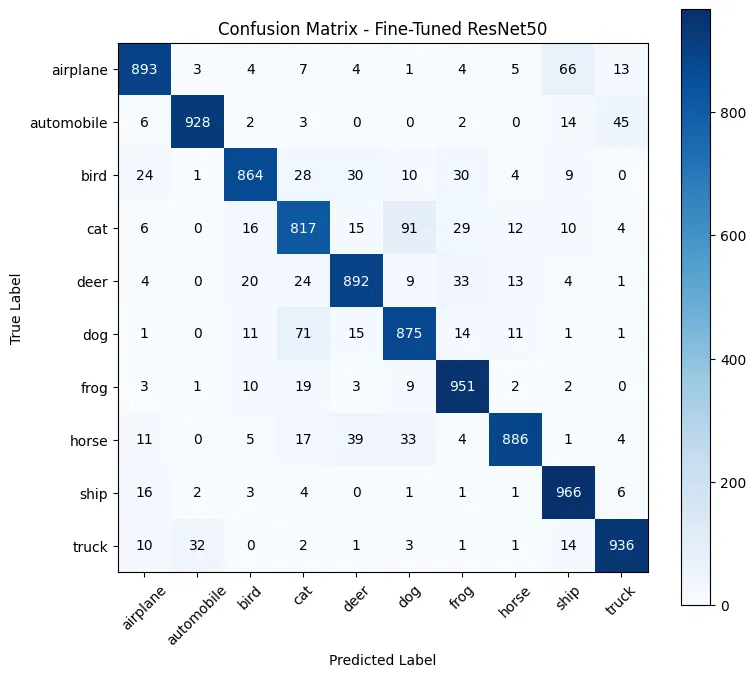
\includegraphics[width=0.8\textwidth]{plot6.png}
\caption{Confusion Matrix of the Fine-Tuned ResNet50 on the CIFAR-10 Testing Set}
\end{figure}

The confusion matrix shows a strong, dominant diagonal across all ten classes, consistent with the 90.08\% overall test accuracy. The most prominent off-diagonal confusions are airplane predicted as ship (66 instances) and truck predicted as automobile (32 instances), both plausible given that airplanes and ships are frequently photographed against similar plain sky or water backgrounds, and automobiles and trucks share a broadly similar boxy silhouette. Cat and dog again show mutual confusion (91 dogs predicted as cat, 71 cats predicted as dog), the same pairing flagged as the model's weakest classes in Section 12.2, while classes such as ship, frog and automobile show very few off-diagonal entries, confirming their high precision and recall.

\vspace{0.15cm}

\subsection*{13.7 Misclassified Images}

\begin{figure}[H]
\centering
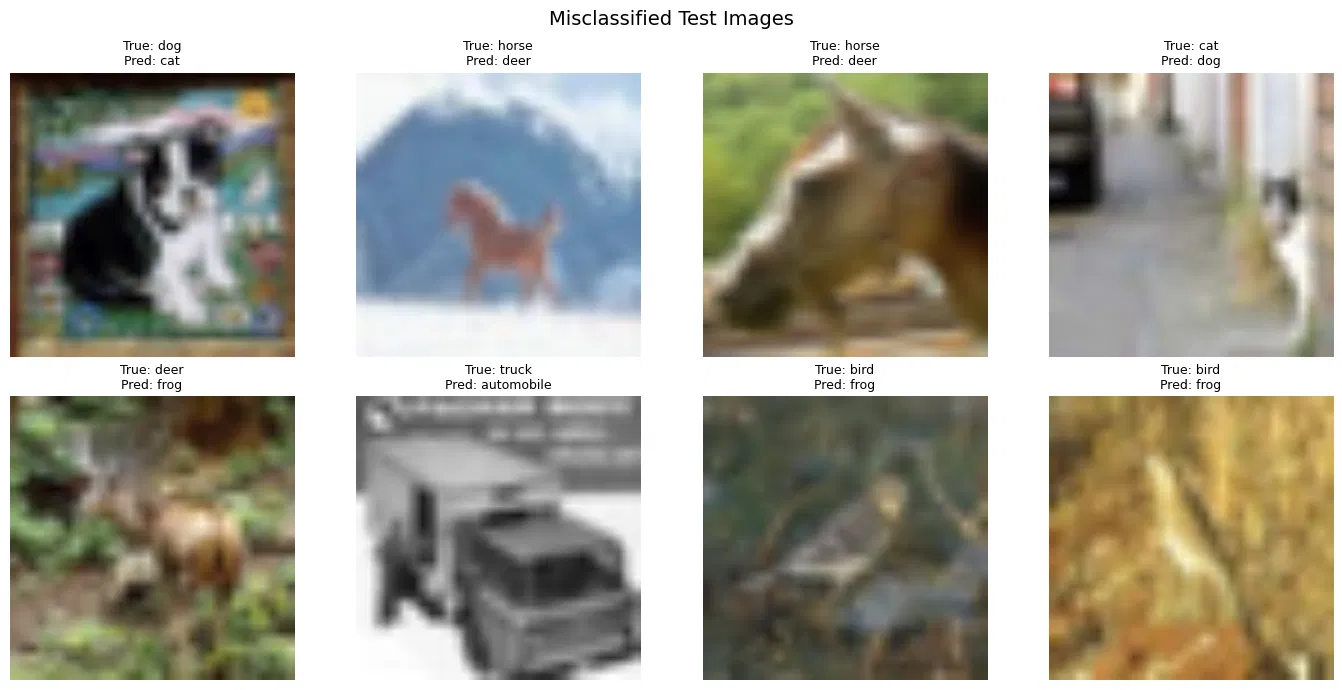
\includegraphics[width=0.95\textwidth]{plot7.png}
\caption{Eight Misclassified Test Images with True and Predicted Labels}
\end{figure}

Several of the misclassified examples are genuinely ambiguous even on visual inspection: a black-and-white dog with a patterned background is confused with cat, and a bird photographed against dense, textured foliage is confused with frog, both plausible errors given the low resolution and close visual similarity between these class pairs. The misclassified truck, photographed at an unusual angle against a light background, is predicted as automobile, again consistent with the vehicle confusion identified in the confusion matrix. These examples suggest that a meaningful share of the model's remaining errors stem from genuine visual ambiguity in the underlying images rather than from a systematic weakness in the learned representation itself.

\section*{14. Result Analysis}

The single most informative comparison in this experiment is between the frozen-backbone baseline and the fine-tuned model: unfreezing just the last residual block of ResNet50 and training it for only 5 further epochs at a reduced learning rate raised validation accuracy from 82.89\% to 90.08\%, a gain of more than 7 percentage points, at the cost of roughly 1,450 additional seconds of training time -- a considerably better return on training time than the 10 epochs spent training the frozen-backbone head alone. Unlike the CNN trained entirely from scratch in Experiment 3, which showed a pronounced 28.8-percentage-point gap between training and testing accuracy indicative of severe overfitting, the fine-tuned ResNet50 model here shows a smaller, though still present, gap of roughly 8.6 percentage points between its final training accuracy (98.68\%) and its test accuracy (90.08\%), suggesting that while some overfitting does occur once layer4 is unfrozen and its 15-million-plus parameters become trainable, the pretrained ImageNet features occupied by the remainder of the frozen backbone provide considerably more regularization than a randomly initialized network of comparable depth would. The macro-averaged Precision, Recall and F1-score of 90.18\%, 90.08\% and 90.07\% respectively are all very close to one another and to the overall accuracy, indicating that performance is fairly balanced across the ten classes rather than being propped up by a small number of especially easy categories, though the cat and dog classes remain the model's clear weak point, mirroring a well-documented difficulty in CIFAR-10 classification generally.

\section*{15. Discussion}

\subsection*{1. Why is AlexNet considered a breakthrough in deep learning?}

AlexNet won the 2012 ImageNet Challenge by a wide margin, proving deep CNNs could outperform traditional computer vision methods at scale. Its use of ReLU activations avoided the vanishing gradients that plagued Sigmoid/Tanh networks, Dropout controlled overfitting in its large fully connected layers, and GPU training made a 61-million-parameter network computationally practical, together reigniting mainstream interest in deep learning.

\subsection*{2. Why does VGG16 use only $3\times3$ convolution filters?}

Stacking multiple $3\times3$ filters achieves the same effective receptive field as a single larger filter (two $3\times3$ layers match a $5\times5$ receptive field) while using fewer parameters and adding an extra non-linearity between them. This uniform, simple design lets VGG16 go deeper than earlier architectures while keeping the network easy to reason about and extend layer by layer.

\subsection*{3. Explain the advantages of the Inception module.}

The Inception module applies $1\times1$, $3\times3$ and $5\times5$ convolutions and pooling in parallel, then concatenates their outputs, capturing multi-scale features at every stage rather than committing to one filter size. Its $1\times1$ convolutions reduce channel depth before expensive larger filters, keeping GoogleNet's parameter count (6.8M) far below AlexNet or VGG16 despite comparable or better accuracy.

\subsection*{4. What is the purpose of residual learning?}

Residual learning reformulates a block's target from the full mapping $H(x)$ to the residual $F(x)=H(x)-x$, added back to the input via a skip connection. This gives gradients a direct path backward through the network regardless of depth, solving the vanishing-gradient problem that previously made networks beyond roughly 20 layers difficult to train.

\subsection*{5. Differentiate LeNet and ResNet.}

LeNet-5 (1998) is a shallow, 7-layer network with only around 60 thousand parameters, using average pooling and no skip connections, designed for simple digit recognition. ResNet (2015) reaches 50 or more layers using residual skip connections that avoid vanishing gradients, achieving far higher accuracy on complex, natural images at the cost of dramatically greater parameter count and computation.

\subsection*{6. What is Transfer Learning?}

Transfer learning reuses a CNN already pretrained on a large dataset such as ImageNet for a new, typically smaller, target task, rather than training from randomly initialized weights. The pretrained convolutional base, which already encodes general-purpose visual features, is frozen and combined with a new classification head suited to the target classes, dramatically reducing the data and compute needed to reach strong accuracy.

\subsection*{7. Why is fine tuning required?}

Training only the new classification head on top of a frozen backbone limits the model to features learned from ImageNet, which may not perfectly match the target dataset's visual characteristics. Fine tuning unfreezes the deepest, most task-specific convolutional layers and retrains them at a small learning rate, letting the pretrained features adapt to the new domain, which in this experiment raised validation accuracy from 82.89\% to 90.08\%.

\subsection*{8. Explain the difference between dilated convolution and transpose convolution.}

Dilated convolution enlarges a kernel's receptive field by inserting gaps between its weights, without changing the input's spatial size or the parameter count, and is used to capture broader context in tasks like segmentation. Transpose convolution instead performs learnable upsampling, increasing a feature map's spatial dimensions, and is used in decoders, GANs and super-resolution where a compact representation must be projected back to full resolution.

\subsection*{9. Why do pretrained models converge faster?}

A pretrained model's convolutional weights already encode general-purpose features -- edges, textures, shapes -- learned from millions of ImageNet images, so training on a new task only needs to adjust or add a much smaller set of task-specific parameters. This was directly visible in this experiment, where the frozen-backbone head's training loss fell from 0.7751 to 0.6143 within the very first two epochs.

\subsection*{10. Compare the computational complexity of LeNet and ResNet.}

LeNet-5 requires only around 60 thousand parameters and correspondingly little computation, since it is shallow and operates on small, low-resolution inputs, making it fast to train even on modest hardware. ResNet50, with roughly 25.6 million parameters spread across 50 layers, requires substantially more computation per forward and backward pass; in this experiment, even with a frozen backbone, a single epoch on 50,000 $224\times224$ images took several minutes on a GPU.

\section*{16. Additional Exercise Solutions}

\subsection*{Exercise 1: Implement transfer learning using VGG16.}

This experiment implemented transfer learning using ResNet50 rather than VGG16, since ResNet50 was selected as the backbone for this run from the four options offered by the lab manual, pairing directly with the ResNet theory covered in Section 4.5. The same overall workflow described in Section 6 -- loading pretrained ImageNet weights, removing the original classifier, freezing the convolutional base, adding a Global Average Pooling layer followed by a Dense layer with ReLU activation and a 10-unit Softmax output, then fine-tuning the last convolutional block -- would apply essentially unchanged if VGG16 were substituted in its place, using \texttt{torchvision.models.vgg16} instead of \texttt{resnet50}. The main practical difference would be VGG16's substantially larger parameter count (138M versus ResNet50's 25.6M), driven mainly by its own large, uniform $3\times3$ convolutional stack and fully connected layers, which would likely increase both training time per epoch and GPU memory requirements relative to the ResNet50 run actually performed here.

\subsection*{Exercise 2: Repeat the experiment using ResNet50.}

ResNet50 was the backbone actually used for the transfer-learning run in this experiment, as described throughout Sections 8 through 12. The frozen-backbone head was trained for 10 epochs using the Adam optimizer at a learning rate of 0.001, reaching a final training accuracy of 84.59\% and a validation accuracy of 82.89\%, before the last convolutional block (\texttt{layer4}) was unfrozen and fine-tuned for a further 5 epochs at a reduced learning rate of 0.0001, raising validation accuracy to 90.08\% and yielding a final test accuracy, on the fully held-out testing set, of 90.08\% with a macro F1-score of 90.07\%. This single run therefore already directly answers this exercise, and the results discussed in Sections 12 and 14 constitute the complete outcome of repeating the experiment with ResNet50 as the chosen architecture.

\subsection*{Exercise 3: Compare Adam and SGD optimizers.}

Only the Adam optimizer was actually used for training in this experiment, as specified in the lab manual's Task 3 configuration and reflected in the hyperparameter study table of Section 10, where the Optimizer = SGD row is explicitly marked as not run. Adam combines per-parameter adaptive learning rates with momentum, typically converging faster than plain SGD in the early epochs of training, which is consistent with the sharp initial drop in training loss (from 0.7751 to 0.6143) observed within the first two frozen-backbone epochs in Section 13.4. SGD, particularly with momentum, can sometimes generalize slightly better over long training runs, but usually requires more careful learning-rate tuning and more epochs to reach comparable accuracy, an experiment that was outside the scope of the single configuration actually trained here.

\subsection*{Exercise 4: Compare training with frozen layers and fine tuning.}

This comparison is directly available from Sections 8, 12.1 and 14 of this report: with the backbone fully frozen, the model reached a validation accuracy of 82.89\% and a validation loss of 0.4952 after 10 epochs, whereas fine-tuning \texttt{layer4} for 5 additional epochs raised validation accuracy to 90.08\% and reduced validation loss to 0.3536. This represents a clear, substantial improvement from fine-tuning relative to training the frozen-backbone head alone, though it comes with an increase in the gap between training and testing accuracy (from roughly 1.7 percentage points in the frozen phase to roughly 8.6 percentage points after fine-tuning), reflecting the trade-off between the greater representational flexibility unlocked by fine-tuning and its correspondingly higher risk of overfitting.

\subsection*{Exercise 5: Evaluate the model using Precision, Recall and F1-score.}

The fine-tuned ResNet50 model was evaluated on the full 10,000-image CIFAR-10 testing set in Section 12.2, achieving a macro-averaged Precision of 90.18\%, Recall of 90.08\% and F1-score of 90.07\%, figures that are all very close to the overall accuracy of 90.08\%, indicating fairly balanced performance across all ten classes rather than a result skewed by a small number of easy categories. The per-class classification report shows this balance is not perfectly uniform, however: automobile and ship both exceed 93\% F1-score, while cat lags well behind at only 82\% F1-score, so the macro average, while broadly representative, still masks a meaningful spread in per-class difficulty.

\subsection*{Exercise 6: Compare the performance of LeNet, AlexNet and ResNet.}

Only ResNet50 was actually trained and evaluated in this experiment, reaching a measured test accuracy of 90.08\% as reported in Section 12.3; LeNet-5 and AlexNet were not trained on CIFAR-10 here, so no directly comparable measured accuracy figures exist for them in this run. Based on the architectural theory covered in Sections 4.1, 4.2 and 4.5, however, LeNet-5's shallow 7-layer design and roughly 60 thousand parameters would be expected to struggle considerably on a natural-image dataset like CIFAR-10 relative to ResNet50's 50-layer, residual-connection architecture, while AlexNet, despite its much larger 61-million parameter count, lacks ResNet's skip connections and would likely be harder to train effectively at comparable depth, making the transfer-learning ResNet50 approach used here the clear practical choice among the three for this dataset.

\section*{17. Conclusion}

A transfer-learning pipeline was built in PyTorch around a pretrained ResNet50 backbone and applied to the CIFAR-10 dataset, loaded from the Hugging Face Hub and resized to $224\times224$ to match the backbone's expected input resolution. The convolutional base was first frozen while a new classification head, consisting of Global Average Pooling followed by a 256-unit Dense layer with ReLU activation and a 10-unit output layer, was trained for 10 epochs using the Adam optimizer, reaching a validation accuracy of 82.89\%; the last residual block of the backbone was then unfrozen and fine-tuned for 5 further epochs at a reduced learning rate of 0.0001, raising validation accuracy to 90.08\% and yielding a final test accuracy of 90.08\%, with macro-averaged Precision, Recall and F1-score of 90.18\%, 90.08\% and 90.07\% respectively. This fine-tuning stage, though comprising only 5 of the 15 total training epochs, contributed the majority of the improvement in generalization performance relative to the frozen-backbone baseline, confirming that adapting even a small, well-chosen subset of a pretrained network's deepest layers can be substantially more valuable than training a small classification head alone. The confusion matrix and misclassified-image inspection identified cat and dog as the model's most persistent source of error, consistent with the visual similarity between these two categories noted throughout the computer vision literature, while classes such as ship, automobile and frog were classified with high reliability. Overall, the experiment reinforced practical understanding of the evolution of CNN architectures, the mechanics and benefits of transfer learning, and the measurable trade-off between the reduced overfitting risk of a frozen backbone and the higher achievable accuracy unlocked by careful fine-tuning.

\section*{18. References}

\begin{enumerate}

\item Yann LeCun,
Leon Bottou,
Yoshua Bengio,
Patrick Haffner,
\textit{Gradient-Based Learning Applied to Document Recognition},
Proceedings of the IEEE,
1998.

\item Alex Krizhevsky,
Ilya Sutskever,
Geoffrey Hinton,
\textit{ImageNet Classification with Deep Convolutional Neural Networks},
NeurIPS,
2012.

\item Karen Simonyan,
Andrew Zisserman,
\textit{Very Deep Convolutional Networks for Large-Scale Image Recognition},
ICLR,
2015.

\item Christian Szegedy et al.,
\textit{Going Deeper with Convolutions},
CVPR,
2015.

\item Kaiming He,
Xiangyu Zhang,
Shaoqing Ren,
Jian Sun,
\textit{Deep Residual Learning for Image Recognition},
CVPR,
2016.

\item Ian Goodfellow,
Yoshua Bengio,
Aaron Courville,
\textit{Deep Learning},
MIT Press,
2016.

\item TensorFlow Documentation.

\url{https://www.tensorflow.org}

\item Keras Documentation.

\url{https://keras.io}

\item PyTorch Documentation.

\url{https://pytorch.org/docs/stable/index.html}

\item TorchVision Models Documentation.

\url{https://pytorch.org/vision/stable/models.html}

\item Hugging Face Datasets Documentation.

\url{https://huggingface.co/docs/datasets}

\end{enumerate}

\vfill

\end{document}
